%%---------------------------------------------------------------------------%%
%% SIAM CSE 2015 Presentation
%%---------------------------------------------------------------------------%%

\documentclass{beamer}
\usefonttheme[onlymath]{serif}
\usepackage{colortbl}
\usepackage{longtable,ltcaption,array}
%% The amssymb package provides various useful mathematical symbols
\usepackage{amssymb}
%% The amsthm package provides extended theorem environments
\usepackage{amsthm} \usepackage{amsmath} \usepackage{tmadd,tmath}
\usepackage{booktabs}
\usepackage{multirow}
\usepackage{caption}
\usepackage[labelformat=empty]{subcaption}
\usepackage{tabularx}

%%---------------------------------------------------------------------------%%
%% THEME SETUP

\usetheme{CambridgeUS}
\usecolortheme{spruce}

%%---------------------------------------------------------------------------%%
%% SETUP STUFF
%%---------------------------------------------------------------------------%%

\logo{
\includegraphics[width=2cm]{new_logo}}

\setbeamercolor{item}{fg=MSUgreen}
\setbeamertemplate{headline}{}
\setbeamertemplate{navigation symbols}{}

\newlength{\DUtablewidth} % internal use in tables

%%---------------------------------------------------------------------------%%
%% MATH STUFF
%%---------------------------------------------------------------------------%%

\newcommand{\Pn}{\textit{P}$\negthinspace_N$}
\newcommand{\SPn}{\textit{SP}$\negthinspace_N$}

\newcommand{\vOmega}{\ensuremath{\ve{\Omega}}}
\newcommand{\hOmega}{\ensuremath{\hat{\ve{\Omega}}}}

\newcommand{\sigs}{\ensuremath{\sigma_{\text{s}}}}
\newcommand{\sigf}{\ensuremath{\sigma_{\text{f}}}}
\newcommand{\sigsm}{\ensuremath{\sigma_{\text{s}m}}}
\newcommand{\sigsn}{\ensuremath{\sigma_{\text{s}n}}}

\newcommand{\phig}{\ensuremath{\Phi}}
\newcommand{\Sigmag}{\ensuremath{\mathbf{\Sigma}}}
\newcommand{\Dg}{\ensuremath{\mathbb{D}}}
\newcommand{\Fg}{\ensuremath{\mathbb{F}}}
\newcommand{\Qg}{\ensuremath{\mathbb{Q}}}
\newcommand{\ug}{\ensuremath{\mathbb{U}}}
\newcommand{\Ag}{\ensuremath{\mathbb{A}}}
\newcommand{\Bg}{\ensuremath{\mathbb{B}}}
\newcommand{\Cg}{\ensuremath{\mathbb{C}}}
\newcommand{\Jg}{\ensuremath{\mathbb{J}}}
\newcommand{\sg}{\ensuremath{\mathbb{S}}}

\newcommand{\aphig}{\ensuremath{\Phi^{\dagger}}}
\newcommand{\aSigmag}{\ensuremath{\mathbf{\Sigma}^{\dagger}}}

\newcommand{\apsi}[1]{\ensuremath{\psi^{\dagger\,#1}}}
\newcommand{\aphi}[1]{\ensuremath{\phi^{\dagger\,#1}}}
\newcommand{\aq}[1]{\ensuremath{q^{\dagger\,#1}}}
\newcommand{\ak}{\ensuremath{k^{\dagger}}}

\newcommand{\normal}{\ensuremath{\hat{\ve{n}}}}

% Phantom minus sign for helping with alignment of matrices
\newcommand{\phmin}{\ensuremath{\phantom{-}}}

\DeclareMathOperator{\diag}{diag}


%%---------------------------------------------------------------------------%%
%% TITLE

\title[Parallel Monte Carlo Solvers]{Parallel Algorithms for Monte Carlo
  Linear Solvers}
\author[Slattery, Hamilton, Evans]{Stuart Slattery
  \\ Steven Hamilton \\ Tom Evans (PI) }
\date[3/17/15]{March 17, 2015}
\institute[ORNL]{\small Oak Ridge National Laboratory}
\titlegraphic{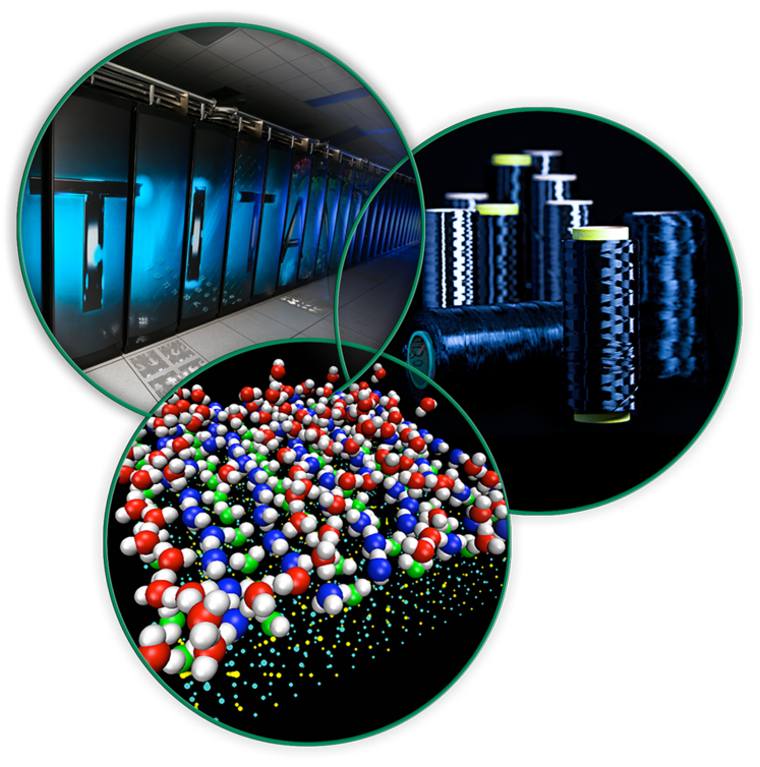
\includegraphics[width=1.5in]{ORNL_Balls.pdf}}

\defbeamertemplate{footline}{titlefoot}{
    \vspace{-0.5cm}
    \hspace*{0.25cm}
    
\includegraphics[width=2cm]{doe_logo}
    \hfill
    
\includegraphics[width=3.25cm]{WordMarkLeaf}
    \hspace*{0.5cm}
}

\setbeamertemplate{title page}
{
  \begin{tabular}{cr}
    \begin{minipage}{4.7cm}
      {\bf \Large\textcolor{MSUgreen}{\inserttitle}}\\

      \vspace{2\baselineskip}
      \insertauthor\\

      \insertinstitute\\

      \insertdate
    \end{minipage}
    &
    \begin{minipage}{5cm}
      \raggedright
      \vspace{-0.75cm}
      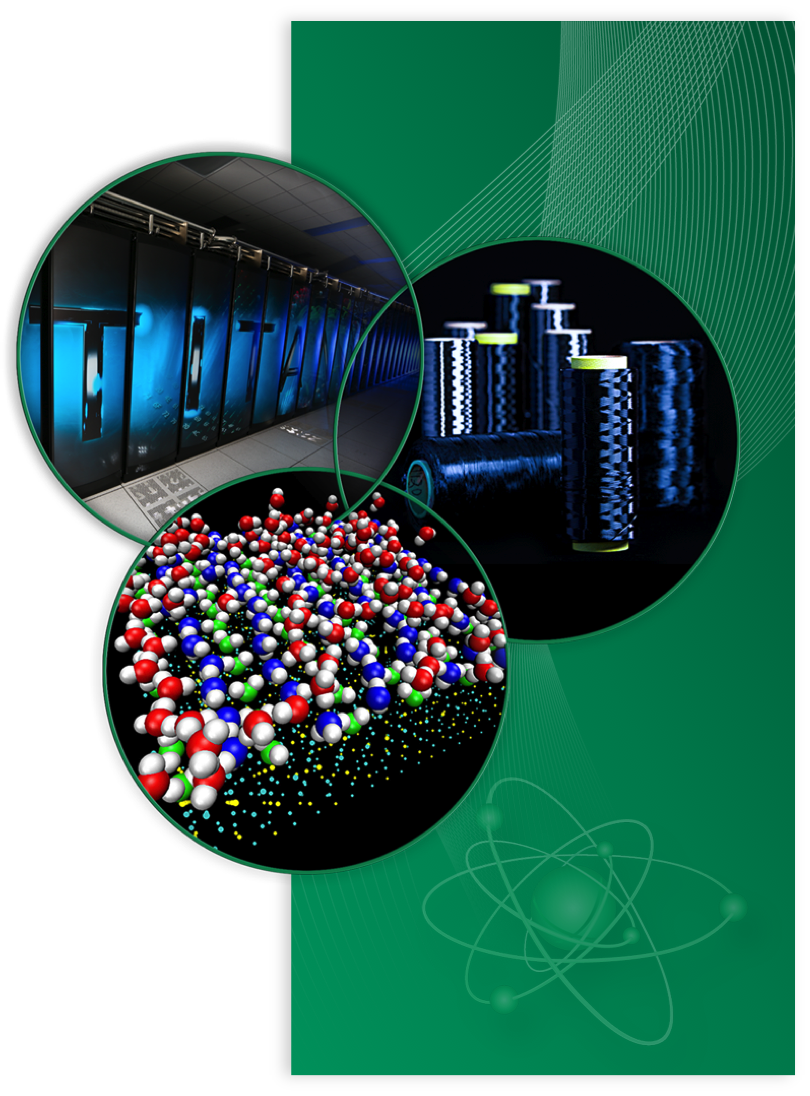
\includegraphics[height=9.8cm]{combined_background}
    \end{minipage}
  \end{tabular}
}

%%---------------------------------------------------------------------------%%
\begin{document}

%%---------------------------------------------------------------------------%%

{
\setbeamertemplate{logo}{}
\setbeamertemplate{footline}[titlefoot]
\begin{frame}
\titlepage
\end{frame}
}

%%---------------------------------------------------------------------------%%
\begin{frame}{Acknowledgments}

  This material is based upon work supported by the U.S. Department of
  Energy, Office of Science, Advanced Scientific Computing Research
  program.

  \vfill

  This research used resources of the Oak Ridge Leadership Computing
  Facility at the Oak Ridge National Laboratory, which is supported by the
  Office of Science of the U.S. Department of Energy under Contract No.
  DE-AC05-00OR22725.

\end{frame}

%%---------------------------------------------------------------------------%%
\begin{frame}{Motivation}
  \vfill
\begin{itemize}
  \item As we move towards exascale computing, the rate of errors is expected
  to increase dramatically
  \vfill
  \begin{itemize}
  \item The probability that a compute node will fail during the course
    of a large scale calculation may be near 1
  \end{itemize}
  \vfill
\item Algorithms need to not only have increased concurrency/scalability
  but have the ability to recover from hardware faults
  \begin{itemize}
  \item Lightweight machines
  \item Heterogeneous machines
  \item Both characterized by low power and high concurrency
  \end{itemize}
  \vfill
\end{itemize}
\vfill
\end{frame}

%%---------------------------------------------------------------------------%%
\begin{frame}{Towards Exascale Concurrency and Resiliency}
  \begin{itemize}
    \item Two basic strategies:
      \vfill
      \begin{enumerate}
        \item Start with current ``state of the art'' methods and make
          incremental modifications to improve scalability and fault
          tolerance
          \begin{itemize}
            \item Many efforts are heading in this direction, attempting
              to find additional concurrency to exploit
          \end{itemize}
        \vfill
        \item Start with methods having natural scalability and resiliency
          aspects and work at improving performance (e.g. Monte Carlo)
          \begin{itemize}
            \item Soft failures introduce an additional stochastic error
              component
            \item Hard failures potentially mitigated by replication
            \item Concurrency enabled by several levels of parallelism
          \end{itemize}
      \end{enumerate}
  \end{itemize}
  \vfill
\end{frame}

%%---------------------------------------------------------------------------%%
\begin{frame}{Outline}

  \begin{itemize}
  \item Monte Carlo Linear Solvers
    \vfill
  \item Domain Decomposition and Replication
    \vfill
  \item Scaling Studies
    \vfill
  \item Algorithm Variations
    \vfill
  \item Conclusions and Future Work
  \end{itemize}
  
\end{frame}

%%---------------------------------------------------------------------------%%
\begin{frame}

  \center Monte Carlo Methods
  
\end{frame}

%%---------------------------------------------------------------------------%%
\begin{frame}{Monte Carlo for Linear Systems}
  \begin{itemize}
    \item Suppose we want to solve $\mathbf{Ax}=\mathbf{b}$
    \vfill
    \item If $\rho(\mathbf{I-A})<1$, we can write the solution using the
      Neumann series
      \begin{equation*}
        \mathbf{x} = \sum_{n=0}^{\infty} (\mathbf{I-A})^n \mathbf{b}
         = \sum_{n=0}^{\infty} \mathbf{H}^n \mathbf{b}
      \end{equation*}
      where $\mathbf{H} \equiv ( \mathbf{I-A} )$ is the Richardson
      iteration matrix 
      \vfill
    \item Build the Neumann series stochastically
  \end{itemize}

  \[
  x_i = \sum_{k=0}^{\infty}\sum_{i_1}^{N}\sum_{i_2}^{N}\ldots
  \sum_{i_k}^{N}h_{i,i_1}h_{i_1,i_2}\ldots h_{i_{k-1},i_k}b_{i_k}
  \]

  \begin{itemize}
  \item Define a sequence of state transitions
  \end{itemize}
  \vspace*{-0.1in}
  \[
  \nu = i \rightarrow i_1 \rightarrow \cdots \rightarrow i_{k-1}
  \rightarrow i_{k}
  \]

\end{frame}

%%---------------------------------------------------------------------------%%
\begin{frame}{Forward Monte Carlo}
\begin{itemize}
  \item Choose a row-stochastic matrix $\mathbf{P}$ and weight matrix
    $\mathbf{W}$ such that $\mathbf{H} = \mathbf{P} \circ \mathbf{W}$
  \item Typical choice (Monte Carlo Almost-Optimal):
    \begin{equation*}
      \mathbf{P}_{ij} = \frac{| \mathbf{H}_{ij}| }
      {\sum_{j=1}^{N} | \mathbf{H}_{ij} | }
    \end{equation*}
  \item To compute solution component $\mathbf{x}_i$:
    \begin{itemize}
      \item Start a history in state $i$ (with initial weight of 1)
      \item Transition to new state $j$ based probabilities determined by
        $\mathbf{P}_i$
      \item Modify history weight based on corresponding entry in
        $\mathbf{W}_{ij}$
      \item Add contribution to $\mathbf{x}_i$ based on current history weight
        and value of $\mathbf{b}_j$
    \end{itemize}
  \item A given random walk can only contribute to a single component of
    the solution vector with $\mathbf{x} \approx \mathbf{M_{MC}} \mathbf{b}$
\end{itemize}
\end{frame}

%%---------------------------------------------------------------------------%%
\begin{frame}{Sampling Example (Forward Monte Carlo)}
  \begin{itemize}
    \item Suppose
  \begin{equation*}
    \mathbf{A} = \begin{bmatrix}
      \phmin 1.0 & -0.2 & -0.6 \\
      -0.4 & \phmin 1.0 & -0.4 \\
      -0.1 & -0.4 & \phmin 1.0 \end{bmatrix} \to
    \mathbf{H} \equiv (\mathbf{I-A}) = \begin{bmatrix}
       0.0 &  0.2 &  0.6 \\
       0.4 &  0.0 &  0.4 \\
       0.1 &  0.4 &  0.0 \end{bmatrix}
  \end{equation*}
    then
  \begin{equation*}
    \mathbf{P} = \begin{bmatrix}
       0.0 & 0.25 & 0.75 \\
       0.5 &  0.0 & 0.5 \\
       0.2 &  0.8 & 0.0 \end{bmatrix}, \quad
    \mathbf{W} = \begin{bmatrix}
       0.0 &  0.8 &  0.8 \\
       0.8 &  0.0 &  0.8 \\
       0.5 &  0.5 &  0.0 \end{bmatrix}
  \end{equation*}
    \vfill
    \item If a history is started in state $3$, there is a $20\%$ chance of
      it transitioning to state $1$ and an $80\%$ chance of moving to state
      $2$
  \end{itemize}
\end{frame}

%%---------------------------------------------------------------------------%%
\begin{frame}{Solving the Heat Equation: Forward Method}

  \begin{figure}[h!]
    \begin{center}
      \includegraphics<1>[width=4in]{direct_1.png}
      \includegraphics<2>[width=4in]{direct_10.png}
      \includegraphics<3>[width=4in]{direct_100.png}
      \includegraphics<4>[width=4in]{direct_1000.png}
    \end{center}
    \caption{
      \only<1>{\textbf{Forward solution.}
        \textit{\sn{2.5}{3} total histories.} }
      \only<2>{\textbf{Forward solution.}
        \textit{\sn{2.5}{4} total histories.} }
      \only<3>{\textbf{Forward solution.}
        \textit{\sn{2.5}{5} total histories.} }
      \only<4>{\textbf{Forward solution.}
        \textit{\sn{2.5}{6} total histories.} }
    }
  \end{figure}

\end{frame}

%%---------------------------------------------------------------------------%%
\begin{frame}

  \center Domain Decomposition and Replication
  
\end{frame}

%%---------------------------------------------------------------------------%%
\begin{frame}{Domain Decomposed Monte Carlo}

  \begin{columns}
    \begin{column}{0.5\textwidth}
      \begin{itemize}
      \item Each parallel process owns a piece of the domain (linear
        system)
        \bigskip
      \item Random walks must be transported between adjacent domains
        through parallel communication
        \bigskip
      \item Domain decomposition determined by the input system
        \bigskip
      \item Load balancing not yet addressed
      \end{itemize}
    \end{column}

    \begin{column}{0.5\textwidth}
      \begin{figure}[htpb!]
        \begin{center}
          \scalebox{0.75}{ \input{ddnu_example.pdftex_t} }
        \end{center}
        \caption{\small Domain decomposition example illustrating
          how domain-to-domain transport creates communication costs.}
      \end{figure}
    \end{column}
  \end{columns}

\end{frame}

%%---------------------------------------------------------------------------%%
\begin{frame}{Asynchronous Monte Carlo Transport Kernel}

  \begin{columns}

    \begin{column}{0.5\textwidth}
      \vspace{-0.1in}
      \small
      \begin{itemize}
      \item General extension of the Milagro algorithm (LANL)
      \item Asynchronous nearest neighbor communication of histories
      \item System-tunable communication parameters of buffer size and check
        frequency (performance impact)
      \item Need an asynchronous strategy for exiting the transport loop
        without a collective (running sum)
      \end{itemize}

      \vspace{-0.1in}
      \begin{figure}[htpb!]
        \begin{center}
          \scalebox{0.45}{ \input{domain_to_domain.pdftex_t} }
        \end{center}
      \end{figure}

    \end{column}

    \begin{column}{0.5\textwidth}

      \vspace{-0.3in}
      \begin{figure}[htpb!]
        \begin{center}
          \scalebox{0.85}{ \input{transport_loop.pdftex_t} }
        \end{center}
      \end{figure}

    \end{column}

  \end{columns}

\end{frame}

%%---------------------------------------------------------------------------%%
\begin{frame}{Exiting the Transport Loop without Collectives}

  \vspace{-0.25in}

  \begin{figure}[htpb!]
    \begin{center}
      \scalebox{0.4}{ \input{master_comm_tree.pdftex_t} }
    \end{center}
    \caption{Master/Slave}
  \end{figure}

  \begin{columns}

    \begin{column}{0.5\textwidth}
      \vspace{-0.75in}
      \begin{figure}[htpb!]
        \begin{center}
          \scalebox{0.4}{ \input{binary_comm_tree.pdftex_t} }
        \end{center}
        \caption{Binary Tree}
      \end{figure}

    \end{column}

    \begin{column}{0.5\textwidth}

      \vspace{-0.5in}
      
      \begin{figure}[t!]
        \begin{center}
          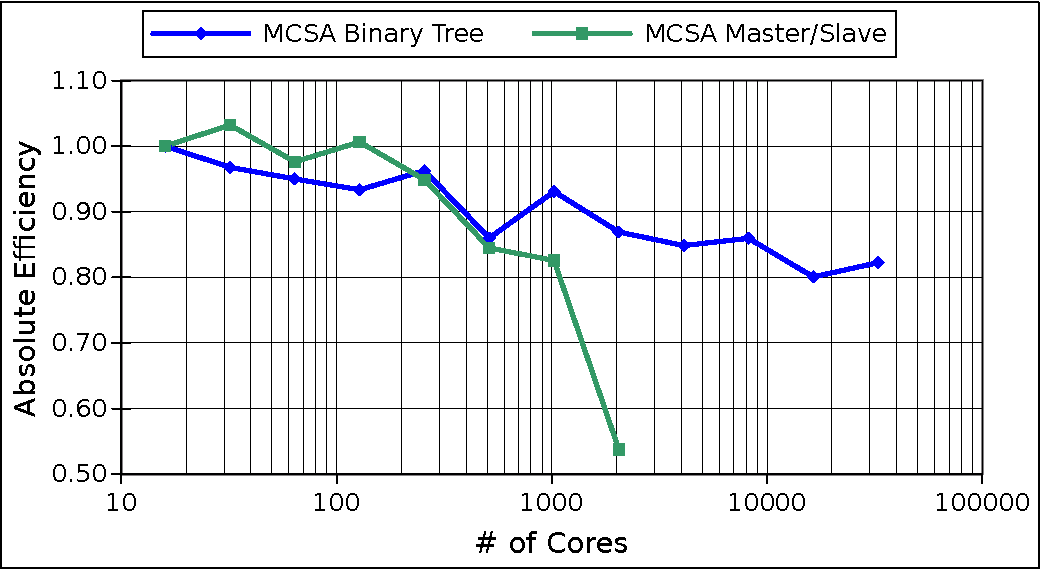
\includegraphics[width=0.99\textwidth]{titan_weak_bvsm.pdf}
        \end{center}
        \caption{Weak scaling absolute efficiency}
        \label{fig:titan_weak_bvsm}
      \end{figure}

    \end{column}

  \end{columns}

\end{frame}

%%---------------------------------------------------------------------------%%
\begin{frame}{Replication}

  Different batches of Monte Carlo samples can be combined in summation via
  superposition if they have different random number streams. For two
  different batches:

  \[
  \mathbf{M_{MC}} \mathbf{x} =
  \frac{1}{2}(\mathbf{M_1}+\mathbf{M_2})\mathbf{x} 
  \]

  Consider each of these batches independent \textit{subsets} of a Monte Carlo
  operator where now the operator can be formed as a general additive
  decomposition of $N_S$ subsets: 

  \[
  \mathbf{M_{MC}} = \frac{1}{N_S}\sum_{n=1}^{N_s}{\mathbf{M_n}}
  \]

  We replicate the linear problem and form each subset on a different group of
  parallel processes. Applying the subsets to a vector requires an AllReduce
  to form the sum. Each subset is domain decomposed.
  
\end{frame}

%%---------------------------------------------------------------------------%%
\begin{frame}

  \center Scaling Studies
  
\end{frame}

%%---------------------------------------------------------------------------%%
\begin{frame}{Parallel Test - Simplified $P_N$ ($SP_N$) Assembly Problem}
\small
\begin{columns}
  
    \begin{column}{0.55\textwidth}

      \vspace{-0.2in}
      \begin{figure}
        \centering
        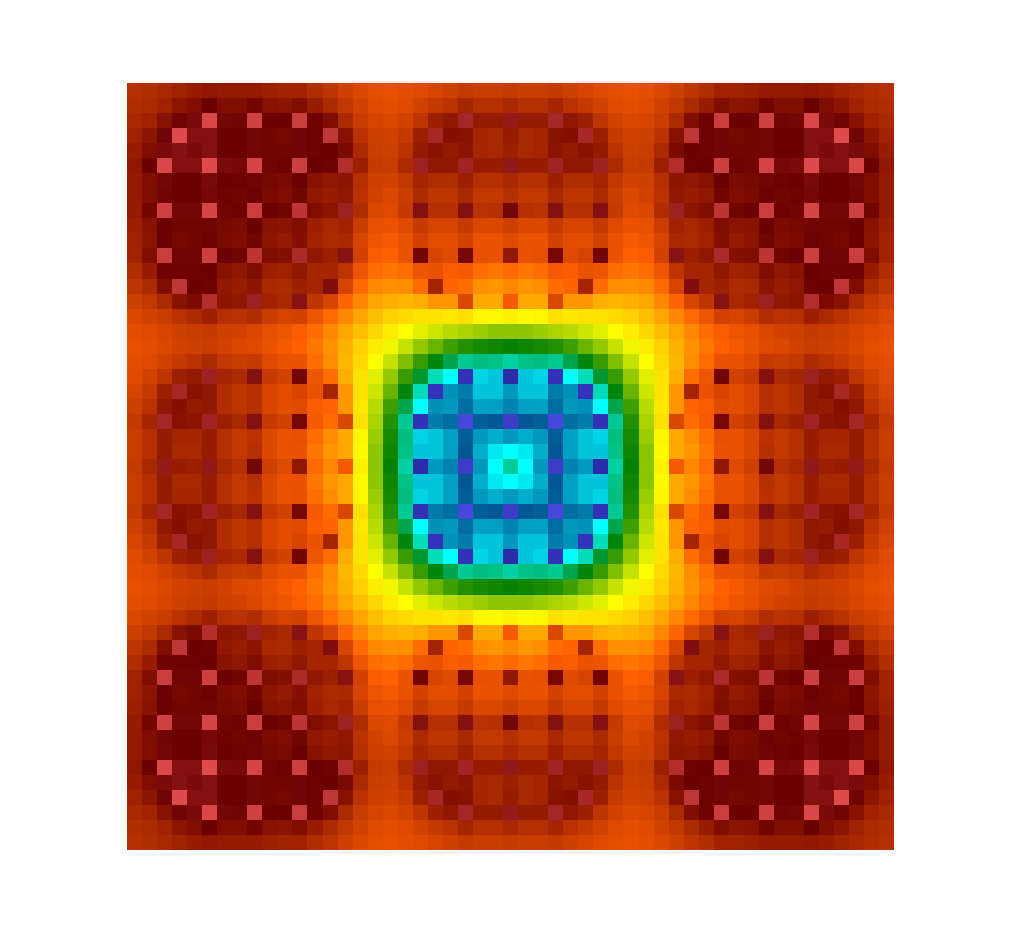
\includegraphics[width=2.0in]{prob4}
        \vspace{-0.2in}
        \caption{$SP_N$ solution example}
      \end{figure}

      The ($SP_N$) equations are an approximation to the Boltzmann neutron
      transport equation used to simulate nuclear reactors

      \vspace{-0.2in}
      
      \[
        \small
        -\nabla \cdot \mathbb{D}_n \nabla \mathbb{U}_n + \sum_{m=1}^4
        \mathbb{A}_{nm} \mathbb{U}_m = \frac{1}{k} \sum_{m=1}^4
        \mathbb{F}_{nm} \mathbb{U}_m
      \]

    \end{column}

    \begin{column}{0.45\textwidth}
      Scaling problem -- $1 \times 1$ to $17 \times 17$ array of fuel
      assemblies with 289 pins each resolved by a $2 \times 2$ spatial mesh
      and 200 axial zones

      \vfill
      
      \begin{itemize}
      \item 7 energy groups, 1 angular moment, 1.6M to 273.5M degrees of
        freedom
      \item 64 to 10,800 computational cores via domain decomposition
      \item We are usually interested in solving generalized eigenvalue
        problem - we use the operator from these problems to test the kernel
        scaling 
      \end{itemize}
    \end{column}
    
  \end{columns}

\end{frame}

%%---------------------------------------------------------------------------%%
\begin{frame}{Monte Carlo Communication Parameters}

  \vspace{-0.15in}
  
  \begin{table}[htb!]
    \begin{center}
      \small
      \begin{tabular}{rr|rrrr}
        \toprule
        \multicolumn{6}{r}{Message Check Frequency} \\
        \multicolumn{1}{r}{} &
        \multicolumn{1}{r}{} &
        \multicolumn{1}{r}{\textbf{128}} &
        \multicolumn{1}{r}{\textbf{256}} &
        \multicolumn{1}{r}{\textbf{512}} &
        \multicolumn{1}{r}{\textbf{1\,024}}
        \\ \midrule
        \multirow{7}{*}{{Message Buffer Size}}
        %%
        & \textbf{256}	& 1.054	& 1.061	& 1.076	& 1.076 \\
        & \textbf{512}	& 1.103	& 1.146	& 1.211	& \framebox[1.1\width]{1.270} \\
        & \textbf{1\,024}	& 1.062	& 1.088	& 1.133	& 1.176 \\
        & \textbf{2\,048}	& 1.030	& 1.042	& 1.072	& 1.107 \\
        & \textbf{4\,096}	& 1.010	& 1.012	& 1.025	& 1.050 \\
        & \textbf{8\,192}	& 1.001	& \framebox[1.1\width]{1.000}	& 1.008	& 1.018 \\
        & \textbf{16\,384}	& 1.017	& 1.003	& 1.010	& 1.009 \\
        %%
        \bottomrule
      \end{tabular}
    \end{center}
  \end{table} 
  \vspace{-0.2in}
  \begin{itemize}
  \item OLCF Eos: 736-node Cray XC30, Intel® Xeon® E5-2670, 11,776
    cores, 47 TB memory, Cray Aries interconnect
  \item 64 cores, 1.6M DOFs, history length of 15, 3 histories per DOF
  \item 27\% decrease in runtime observed for bad parameter choices
  \item Worth the time to do this parameter study when running on new
    hardware
  \end{itemize}
  
\end{frame}

%%---------------------------------------------------------------------------%%
\begin{frame}{Monte Carlo Scaling}

  \vspace{-0.1in}
  
  \begin{table}[htb!]
    \tiny
    \begin{center}
      \begin{tabular}{rrrrrrr}
        \toprule
        \multicolumn{1}{r}{Cores} &
        \multicolumn{1}{r}{DOFs} &
        \multicolumn{1}{r}{DOFs/Core} &
        \multicolumn{1}{r}{Time Min (s)} &
        \multicolumn{1}{r}{Time Max (s)} &
        \multicolumn{1}{r}{Time Ave (s)} &
        \multicolumn{1}{r}{Efficiency}
        \\ \midrule
        %%
        256 & 273\,509\,600 & 1\,068\,397 & 260.53 & 260.54 & 260.54 & 1.00 \\
        1\,024 & 273\,509\,600 & 267\,099 & & & & \\
        4\,096 & 273\,509\,600 & 66\,775 & & & & \\
        7\,744 & 273\,509\,600 & 35\,319 & & & & \\
        10\,816 & 273\,509\,600 & 25\,288 & & & & \\
        %%
        \bottomrule
      \end{tabular}
    \end{center}
    \vspace{-0.09in}
    \caption{\small Strong Scaling}
  \end{table} 

  \vspace{-0.2in}
  
  \begin{table}[htb!]
    \tiny
    \begin{center}
      \begin{tabular}{rrrrrrr}
        \toprule
        \multicolumn{1}{r}{Cores} &
        \multicolumn{1}{r}{DOFs} &
        \multicolumn{1}{r}{DOFs/Core} &
        \multicolumn{1}{r}{Time Min (s)} &
        \multicolumn{1}{r}{Time Max (s)} &
        \multicolumn{1}{r}{Time Ave (s)} &
        \multicolumn{1}{r}{Efficiency}
        \\ \midrule
        %%
        64 & 1\,618\,400 & 25\,288 & 6.432 & 6.432 & 6.432 & 1.00 \\
        256 & 6\,473\,600 & 25\,288 & 6.493 & 6.493 & 6.493 & 0.99 \\
        1\,024 & & 25\,288 & & & & \\
        4\,096 & & 25\,288 & & & & \\
        7\,744 & & 25\,288 & & & & \\
        10\,816 & & 25\,288 & & & & \\
        %
        \bottomrule
      \end{tabular}
    \end{center}
    \vspace{-0.09in}
    \caption{\small Weak Scaling}
  \end{table}

  \vspace{-0.2in}

  \begin{table}[htb!]
    \tiny
    \begin{center}
      \begin{tabular}{rrrrrrr}
        \toprule
        \multicolumn{1}{r}{Subsets} &
        \multicolumn{1}{r}{Cores} &
        \multicolumn{1}{r}{DOFs} &
        \multicolumn{1}{r}{Time Min (s)} &
        \multicolumn{1}{r}{Time Max (s)} &
        \multicolumn{1}{r}{Time Ave (s)} &
        \multicolumn{1}{r}{Efficiency}
        \\ \midrule
        %%
        1 & 256 & 6\,473\,600 & 6.493 & 6.493 & 6.493 & 1.00 \\
        2 & 512 & 6\,473\,600 &  &  & & \\
        3 & 768 & 6\,473\,600 &  &  & & \\
        4 & 1\,024 & 6\,473\,600 & &  & & \\
        %
        \bottomrule
      \end{tabular}
    \end{center}
    \vspace{-0.09in}
    \caption{\small Replication Scaling. 256 cores per subset.}
  \end{table} 

\end{frame}

%%---------------------------------------------------------------------------%%
\begin{frame}

  \center Algorithm Variations
  
\end{frame}

%%---------------------------------------------------------------------------%%
\begin{frame}{Monte Carlo Synthetic Acceleration (MCSA)}
  \begin{itemize}
  \item Devised by Evans and Mosher in the 2000's as an acceleration
    scheme for radiation diffusion problems (LANL)
    \vfill
  \item Can be abstracted as a general linear solver with Monte Carlo as a
    preconditioner
    \vfill
  \item First Richardson step hits the high frequency error modes and second
    Monte Carlo step hits the low frequency error modes
  \end{itemize}
  \vfill
  \begin{align*}
    \mathbf{r}^k &= \mathbf{b} - \mathbf{Ax}^k \\
    \mathbf{x}^{k+1/2} &= \mathbf{x}^k + \mathbf{r}^k \\
    \mathbf{r}^{k+1/2} &= \mathbf{b} - \mathbf{Ax}^{k+1/2} \\
    \mathbf{x}^{k+1} &= \mathbf{x}^{k+1/2} + \mathbf{M_{MC}} \mathbf{r}^{k+1/2}
  \end{align*}
\end{frame}

%%---------------------------------------------------------------------------%%
\begin{frame}{Matrix-Free Algorithm}

  \begin{columns}
    
    \begin{column}{0.4\textwidth}
      
      \begin{itemize}
        \small
      \item At each application of $\mathbf{M_{MC}}$, execute the Monte
        Carlo process
        \vfill
      \item Must perform Monte Carlo every time you want to apply with a better
        approximation requiring more time and more operations
        \vfill
      \item Variations in random number streams are amortized over iterations
        \vfill
      \item Vast majority of solve time spent doing Monte Carlo
      \end{itemize}

    \end{column}

    \begin{column}{0.6\textwidth}
      \begin{table}[htb!]
        \tiny
        \begin{center}
          \begin{tabular}{rrrrr}
            \toprule
            \multicolumn{1}{r}{$L$} &
            \multicolumn{1}{r}{$N_S$} &
            \multicolumn{1}{r}{MC Time (s)} &
            \multicolumn{1}{r}{MC Fraction} &
            \multicolumn{1}{r}{MCSA Iters}
            \\ \midrule
            %%
            3 & 1 & 30.885 & 0.96 & 266 \\
            3 & 2 & 60.869 & 0.98 & 261 \\
            5 & 1 & 27.422 & 0.97 & 180 \\
            5 & 2 & 54.319 & 0.98 & 175 \\
            10 & 1 & 23.871 & 0.98 & 102 \\
            10 & 2 & 45.551 & 0.99 & 97 \\
            15 & 1 & 50.395 & 0.98 & 164 \\
            15 & 2 & 42.951 & 0.99 & 69 \\
            15 & 3 & 65.292 & 0.99 & 68 \\
            25 & 1 & - & - & - \\
            25 & 2 & 70.505 & 0.99 & 78 \\
            25 & 3 & 63.677 & 1.00 & 47 \\
            %
            \bottomrule
          \end{tabular}
        \end{center}
        \caption{\small MCSA performance. $A$ had $115\,600$ rows and
          $1\,186\,464$ non-zero entries.}
      \end{table} 

    \end{column}
  \end{columns}
  
\end{frame}

%%---------------------------------------------------------------------------%%
\begin{frame}{Stochastic Approximate Inverse Algorithm}

  \vspace{-0.1in}
  
  \begin{itemize}
    \small
    \item Construct $\mathbf{M_{MC}}$ as a sparse matrix by executing the
      Monte Carlo process once and tallying the row entries
    \item Use this operator as a stochastic approximation to the inverse
    \item A better approximation to the inverse requires more setup time and
      more storage
    \item We will investigate a drop tolerance strategy to control sparsity
  \end{itemize}

  \vspace{-0.1in}

  \begin{table}[htb!]
    \tiny
    \begin{center}
      \begin{tabular}{rrrrrrr}
        \toprule
        \multicolumn{1}{r}{$L$} &
        \multicolumn{1}{r}{$N_S$} &
        \multicolumn{1}{r}{$NNZ$} &
        \multicolumn{1}{r}{$NNZ$ Ratio} &
        \multicolumn{1}{r}{MC Time (s)} &
        \multicolumn{1}{r}{Setup Time (s)} &
        \multicolumn{1}{r}{MCSA Iters}
        \\ \midrule
        %%
        3 & 2 & 484\,714 & 0.41 & 0.104 & 0.671 & 255 \\
        3 & 3 & 622\,123 & 0.52 & 0.145 & 0.705 & 255 \\
        5 & 2 & 783\,153 & 0.66 & 0.158 & 0.737 & 185 \\
        5 & 3 & 1\,032\,573 & 0.87 & 0.237 & 0.831 & 171 \\
        5 & 4 & 1\,241\,442 & 1.05 & 0.302 & 0.906 & 171 \\
        10 & 3 & 1\,969\,540 & 1.66 & 0.433 & 1.061 & 95 \\
        10 & 4 & 2\,416\,572 & 2.04 & 0.570 & 1.214 & 95 \\
        15 & 3 & 2\,867\,005 & 2.42 & 0.645 & 1.317 & 132 \\
        15 & 4 & 3\,544\,181 & 2.99 & 0.833 & 1.534 & 67 \\
        15 & 5 & 4\,157\,269 & 3.50 & 1.029 & 1.765 & 66 \\
        \bottomrule
      \end{tabular}
    \end{center}
    \caption{MCSA Performance. $A$ had $115\,600$ rows and $1\,186\,464$
      non-zero entries.}
  \end{table} 

\end{frame}

%%---------------------------------------------------------------------------%%
\begin{frame}{Unpreconditioned Algorithm Comparison}

  \begin{itemize}
    \small
  \item No preconditioning, serial computation, fastest MCSA times reported
  \item GMRES easier to preconditioner - performance here only indicates Monte
    Carlo potential
  \item These results indicate good stochastic approximate inverse performance
    for traditional CPU architectures
  \item Matrix-free approach may be more effective when vectorized for new
    architectures by favoring operations over storage - 95\%+ of the runtime
    spent in Monte Carlo
  \end{itemize}

  \begin{table}[htb!]
    \tiny
    \begin{center}
      \begin{tabular}{lrrrr}
        \toprule
        \multicolumn{1}{l}{Solver} &
        \multicolumn{1}{r}{Setup Time (s)} &
        \multicolumn{1}{r}{Solve Time (s)} &
        \multicolumn{1}{r}{Total Time (s)} &
        \multicolumn{1}{r}{Iters}
        \\ \midrule
        %%
        MCSA Matrix-Free & 2.104 & 24.389 & 26.493 & 102 \\
        MCSA Approximate Inverse & 2.953 & 0.779 & 3.731 & 95 \\
        Belos GMRES & 1.791 & 1.021 & 2.812 & 81\\
        %
        \bottomrule 
      \end{tabular}
    \end{center}
    \caption{$A$ had $115\,600$ rows and $1\,186\,464$ non-zero entries.}
  \end{table} 

\end{frame}

%%---------------------------------------------------------------------------%%
\begin{frame}

  \center Conclusions and Future Work
  
\end{frame}

%%---------------------------------------------------------------------------%%
\begin{frame}{Conclusions}
  \begin{itemize}
  \item Monte Carlo methods offer great potential for both resilient and
    highly parallel solvers
    \vfill
  \item A fully asynchronous algorithm provides a scheme without collectives 
    \vfill
  \item Good scaling demonstrated so far on reasonably load balanced problems
    \vfill
  \item Replication a potential resiliency strategy with some overhead
    \vfill
  \item Matrix-free and stochastic approximate inverse algorithms are
    complementary - trade operations for storage
  \end{itemize}
\end{frame}

%%---------------------------------------------------------------------------%%
\begin{frame}{Current and Future Work}
  \begin{itemize}
  \item Vectorization an area of active research with a focus on heterogeneous
    architectures (Titan and Summit)
    \vfill
  \item Multiple threading models are being explored (Kokkos, HPX, etc.)
    \vfill
  \item Extending methods to broader problem areas is significant algorithmic
    challenge and an attractive area for continued research
    \vfill
  \item Performance modeling and resiliency simulations this FY
  \end{itemize}
\end{frame}

%%---------------------------------------------------------------------------%%
\end{document}
%%---------------------------------------------------------------------------%%

%%---------------------------------------------------------------------------%%
%% end of pres.tex
%%---------------------------------------------------------------------------%%
